%\documentclass[times, 12pt, twocolumn]{article}
\documentclass[times, 12pt]{article}

% Config
\usepackage{caption}
\usepackage{url}
\usepackage{graphicx}
\usepackage{attachfile}
\usepackage{hyperref}
\usepackage{pdfpages}
\usepackage{appendix}
\usepackage{glossaries}
\usepackage{subfigure}
\usepackage{subcaption}


\usepackage{times} % Use Times New Roman font
\usepackage{setspace} % For setting line spacing
\usepackage{enumitem} % For customizing enumerations
\usepackage{float} % For placing images


%\usepackage{blindtext}
%\usepackage{lipsum}
%\usepackage[a4paper, total={6in, 8in}]{geometry}
%\usepackage[pass, showframe]{geometry}

\newcommand{\schooladdress}{
  \textbf{ENSSAT LANNION} \\
  6 rue Kerampont \\
  22300 LANNION\\
  FRANCE
}

\newcommand{\documenttitle}{
  Rapport de Projet de Bases de Données Avancées
}

\newcommand{\documentsubtitle}{
  Analyse de résumés de données
}

\newcommand{\studentinfo}{
  Mattias Kockum \\
  Informatique - ENSSAT Promotion 2023
}

\newcommand{\schooltutor}{
  \textbf{Enseignant ENSSAT} Olivier Pivert 
}

\newcommand{\dates}{
  \today{}
}

\renewcommand{\contentsname}{Table des matières}
\renewcommand{\listfigurename}{Table des figures}
\renewcommand{\listtablename}{Table des tableaux}
\renewcommand{\glossaryname}{Glossaire}
\renewcommand{\refname}{Bibliographie}



\hypersetup{
    colorlinks=true,
    linkcolor=blue,
    filecolor=magenta,
    urlcolor=cyan,
    pdfborder={0 0 0},
}

% Customizations for enumerations
\setlist[enumerate]{align=left, labelsep=1em}

% Line spacing
\onehalfspacing

% Justify text
\raggedright

\input{annexes/glossary}


\begin{document}
% Introduction
\begin{titlepage}
    \centering
    % Company logo on the left
    \begin{minipage}[t]{0.4\textwidth}
        \raggedright
        %\includegraphics[width=0.8\linewidth]{images/company_logo.png}
        
        \vspace{0.5cm}
        %\companyaddress
    \end{minipage}
    \hfill % Fill the space between the logos
    % School logo on the right
    \begin{minipage}[t]{0.4\textwidth}
        \raggedleft
        
\includegraphics[width=0.8\linewidth, height=2cm]{images/school_logo.png}
        
        \vspace{0.5cm}
        \schooladdress
    \end{minipage}

    \vspace{2cm}

    \Large
    \documenttitle \\
    \vspace{1cm}
    \Huge
    \textbf{\documentsubtitle} \\
    \normalsize
    %\documentsubtitleenglish \\
    \vspace{1cm}
    \studentinfo \\
    \vspace{1cm}
    %\companytutor \\
    \schooltutor \\
    \vspace{1cm}
    \dates \\
    \vfill

\end{titlepage}

\tableofcontents
%\listoffigures
\section{Introduction}
  Notre travail consiste à étudier des résumés de données.
  Ces résumés de données sont obtenus grâce à une réécriture d'une base de données classique concernant des millions de vols commerciaux américains.
  Le code utilisé est une adaptation du code proposé en cours.
  Pour notre analyse, nous avons choisi d'utiliser un sous ensemble des données brutes, bien que l'utilisateur final ait la possibilité d'utiliser toutes ses données en entrée du programme.
  Nous avons produit un programme agencé autour d'un 'main.py' qui orchestre les trois parties du programme : l'extraction de sous ensemble, la réécriture en données floues, et l'analyse de ces données.

% Corps
\section{Réécriture}
  Dans cette première partie, nous avons écrit le code permettant de calculer les moyennes des données et de les sauvegarder au format JSON.
  Nous avons aussi écrit les fonctions permettant de visualiser l'équilibre des termes.
  Pour cela, nous regardons la satisfaction moyenne de chaque modalité d'un même terme sur l'ensemble des données.
  Cela permet de savoir si une des modalités prend le pas sur les autres. [fig:\ref{fig:balance}]

\begin{figure}[H]
  \centering
  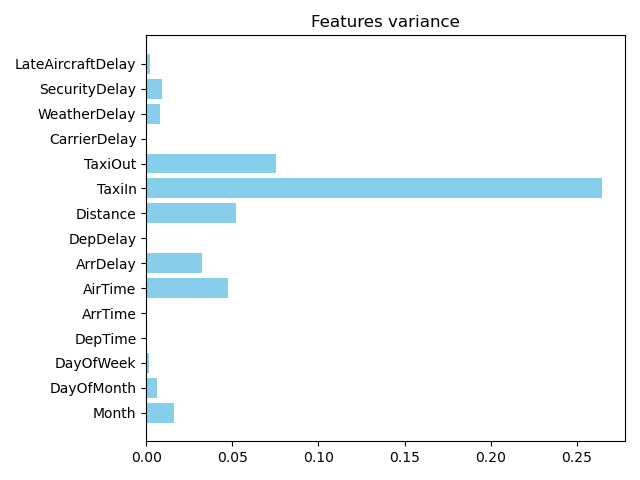
\includegraphics[scale=1]{images/balance_figure.png}
  \caption{}
  \label{fig:balance}
\end{figure}

Dans certains cas, cela semble cohérent avec des variations auxquelles on peut s'attendre Par exemple : Plus d'avions lors des vacances d'été et d'hiver [fig:\ref{fig:Month}] ou un équilibre entre les jours du mois. [fig:\ref{fig:DayOfMonth}]

\begin{figure}[H]
  \centering
  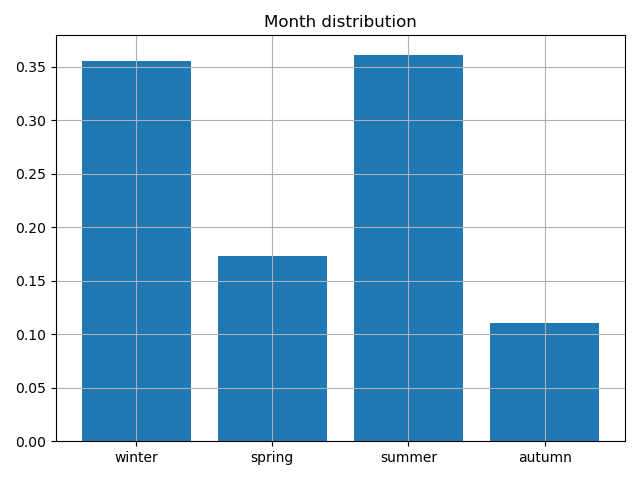
\includegraphics[scale=1]{images/Month_distribution.png}
  \caption{}
  \label{fig:Month}
\end{figure}

\begin{figure}[H]
  \centering
  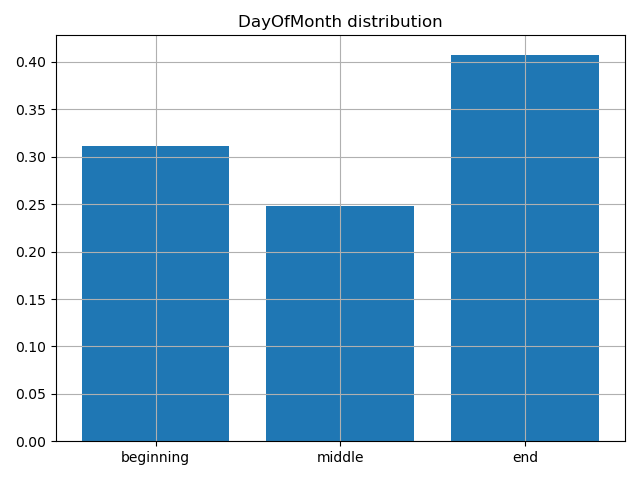
\includegraphics[scale=1]{images/DayOfMonth_distribution.png}
  \caption{}
  \label{fig:DayOfMonth}
\end{figure}

Dans d'autres cas, cela peut être plus étonnant. [fig:\ref{fig:TaxiIn}]
Ici, dans le cas des taxis cela peut indiquer, soit que les taxis déposent très rapidement les voyageurs, ce qui est possible, soit que les classes sont mal définies.
En effet, la modalité 'short' de 'TaxiIn' va jusqu'à 20 minutes d'attente, il serait donc potentiellement judicieux de rajouter une modalité intermédiaire à 'short' et 'medium' pour augmenter la granularité de la donnée, augmenter sa précision et son équilibre.

\begin{figure}[H]
  \centering
  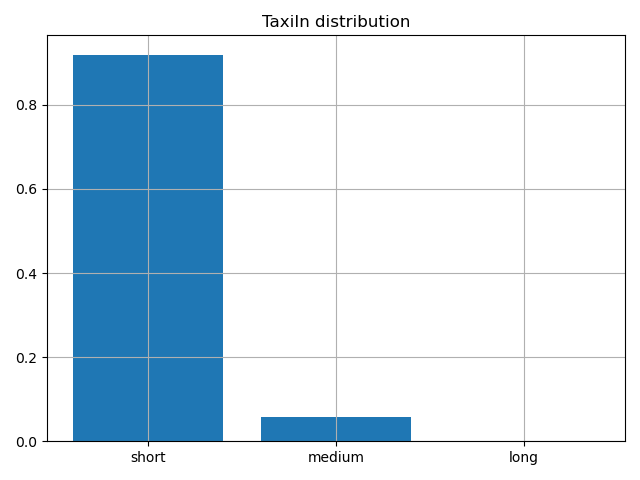
\includegraphics[scale=1]{images/TaxiIn_distribution.png}
  \caption{}
  \label{fig:TaxiIn}
\end{figure}


\input{sections/exploration_des_données}
\section{Termes corrélés}
  Pour identifier les termes corrélés, nous avons opté pour une matrice de corrélation.
  Ici, la bibliothèque pandas permet d'effectuer le calcul de la corrélation sur tout le tableau.

\begin{figure}[H]
  \centering
  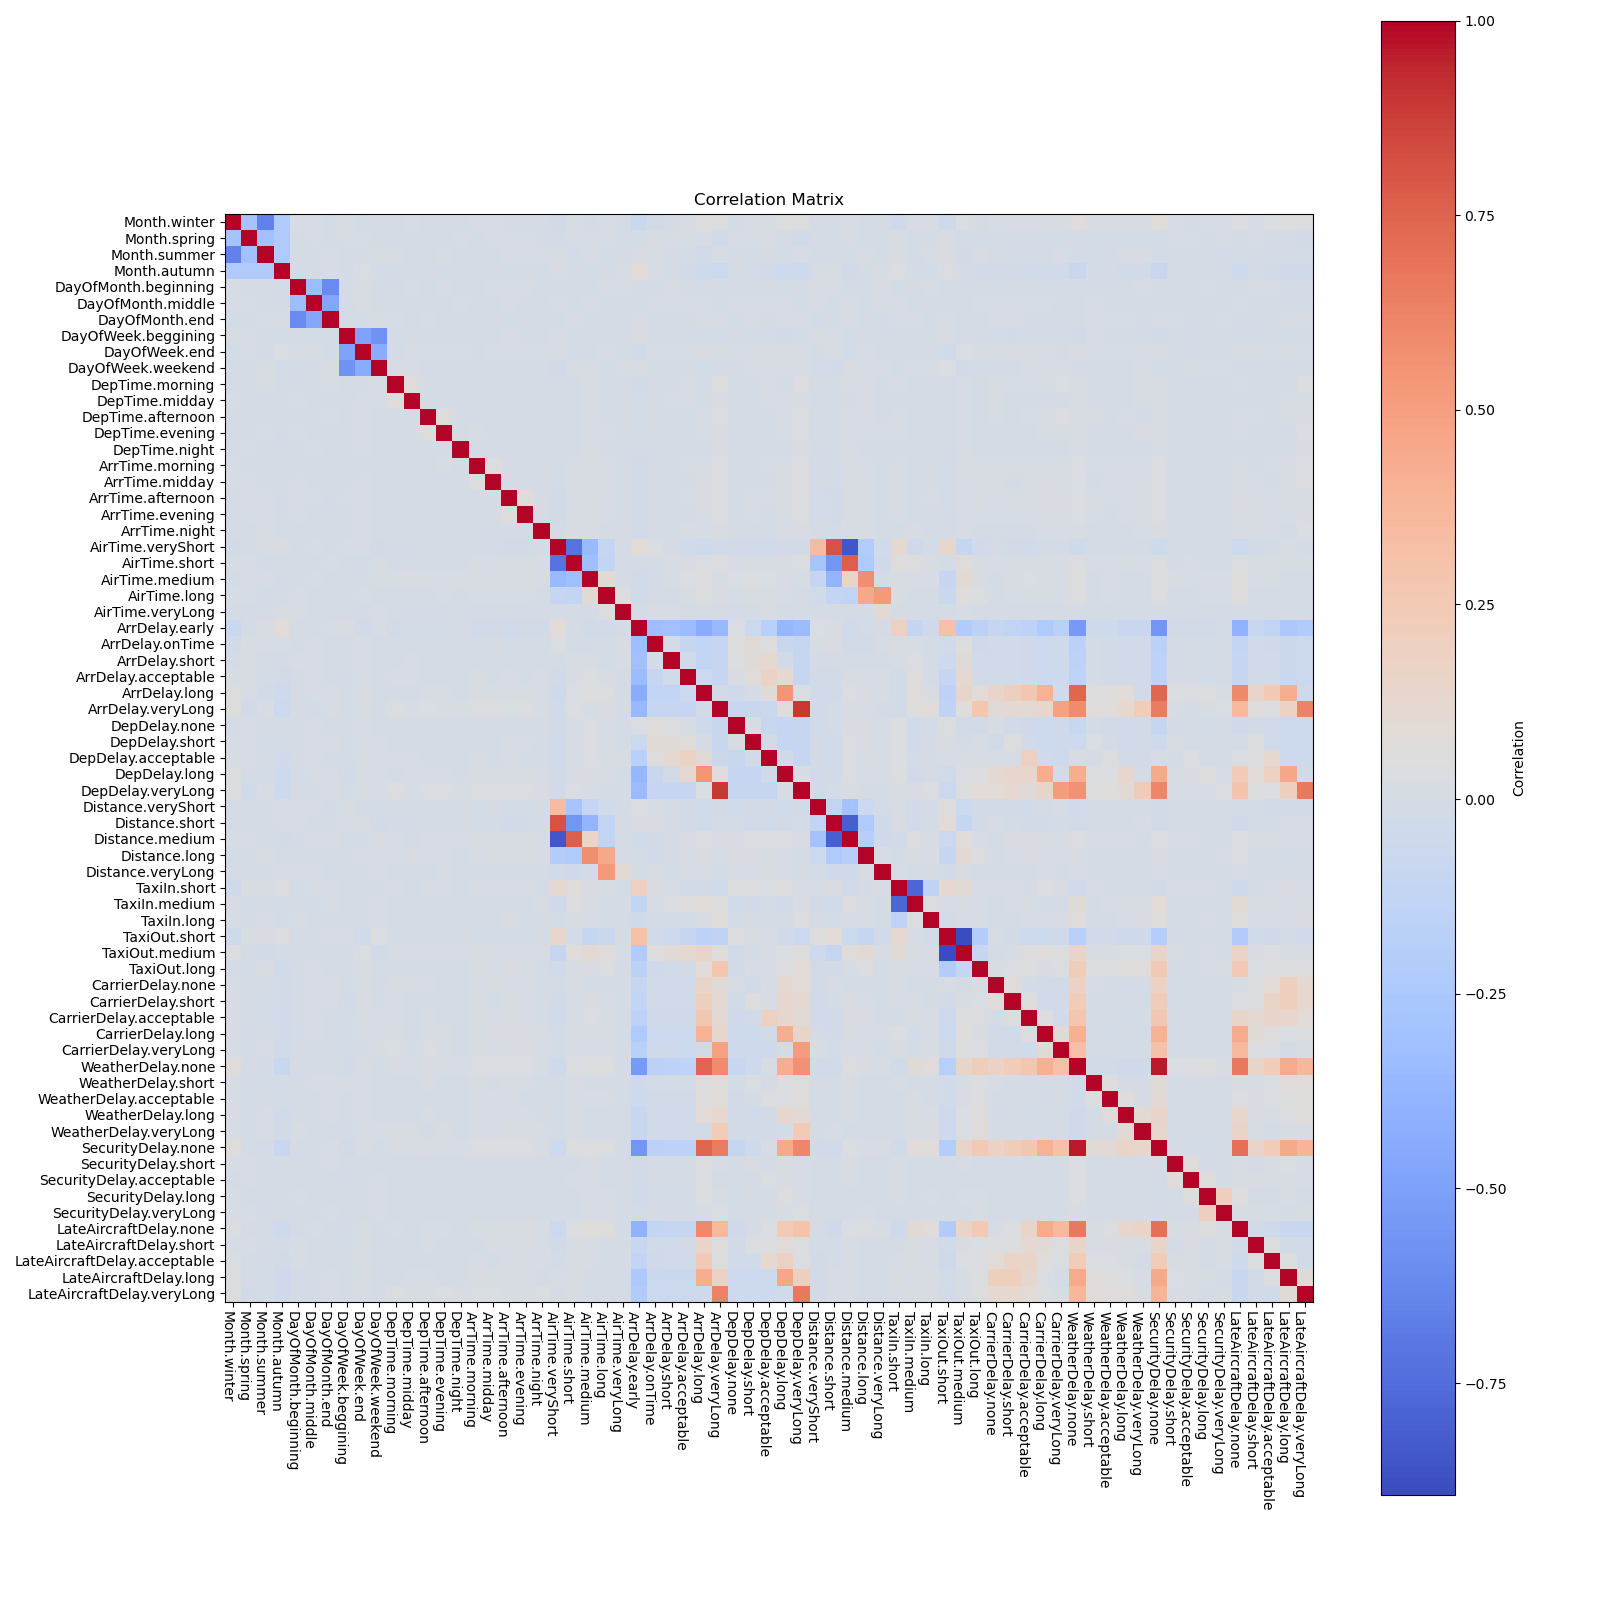
\includegraphics[scale=0.45]{images/correlation_matrix.png}
  \caption{}
  \label{fig:correlation}
\end{figure}

Sur la matrice de corrélation obtenue [fig:\ref{fig:correlation}], nous pouvons encore une fois observée des choses qui étaient attendues, comme le fait que 'AirTime.veryShort' soit positivement corrélé à 'Distance.short' et négativement à 'Distance.medium'.

\section{Termes atypiques}
  Pour identifier les termes atypiques, nous avons réutilisé le code vu précédemment pour obtenir l'équilibre des modalités.
  De cette manière, nous pouvons par exemple identifier que les départs de nuit sont peu fréquents. [fig:\ref{fig:DepTime}]

\begin{figure}[H]
  \centering
  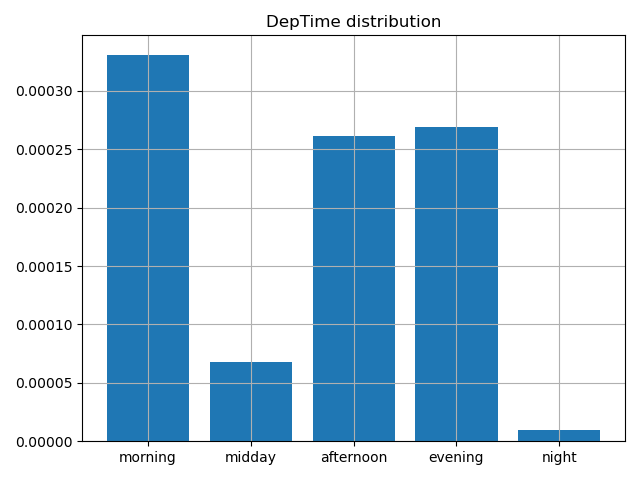
\includegraphics[scale=1]{images/DepTime_distribution.png}
  \caption{}
  \label{fig:DepTime}
\end{figure}


% Bibliographie
%\bibliographystyle{plain}
%\bibliography{references/bibliography}
%\addcontentsline{toc}{section}{Bibliographie}
% Annexes
%\appendix
%\printglossaries
%\addcontentsline{toc}{section}{Glossaire}
%\input{annexes/annexes}

\end{document}


